\frontchapter{Chapitres Liminaires}
\begingroup\small\setstretch{1.05}\origpage{15}{001}
Gravir une montagne ne s’improvise pas : il est impératif de bien se préparer. Excès de confiance ou de précipitation, manque d’échauffement ou de direction, et c’est le découragement et l’abandon assurés. De même, pour le lecteur ou la lectrice novice, ce livre imposant à de quoi impressionner.\ednote{原文 « à de quoi » 应为 « a de quoi »，此处为动词 avoir，而非介词 à。} Avant donc que d’attaquer de front ce qui en constitue l’objet, à savoir les sciences du langage, je vous propose une « marche d’approche », un échauffement, en quelque sorte, sous la forme de deux chapitres introductifs. Les deux questions qui y posées sont\ednote{原文如此；关系从句缺少助动词 « sont »，应作 « Les deux questions qui y sont posées sont très simples »。} très simples, pleines de bon sens. Tout étudiant en langues étrangères, mais aussi tout être humain en général, devrait se les poser.
\begin{center}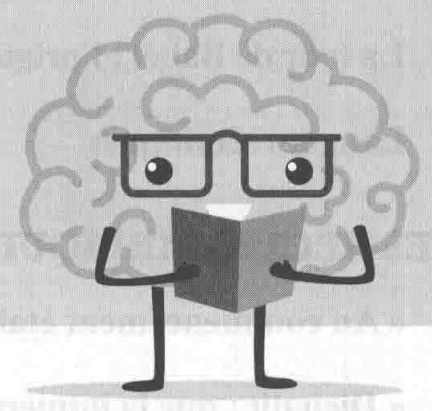
\includegraphics[width=22mm]{assets/liminaires_illustration.png}\end{center}
\minititle{Le chapitre 1}
« Existe-t-il une langue originelle ? » nous nous poserons la question de l’origine du langage. Cette question, vieille comme le monde, si je puis dire, n’a cessé de faire polémique chez les linguistes : certains la jugent essentielle, d’autres la jugent inutile, au point d’avoir même interdit toute publication à ce sujet pendant de nombreuses années. Fort heureusement, cette interdiction été levée depuis peu,\ednote{原文 « cette interdiction été levée » 缺少助动词 « a »，应为 « cette interdiction a été levée »。} et la question de l’origine du langage connaît un grand regain d’intérêt de nos jours\origfoot{1}{Citons par exemple \textit{La langue d’Adam} (2010), du linguiste américain Derek Bickerton (1926-2018).}. Les récits bibliques, la philosophie (Aristote, Rousseau, Voltaire, etc.) mais aussi les sciences modernes (paléontologie, génétique, paléogénétique, etc.) viendront nous apporter des réponses à travers leur découvertes les plus récentes.\ednote{原文 « leur découvertes » 应为 « leurs découvertes »，限定词与复数名词保持一致。}
\minititle{Le chapitre 2}
« Le langage est-il le propre de l’homme ? » nous nous poserons une question bien connue elle aussi. Est-il vrai de dire « 鸟有鸟语，人有人言 »? Pour tracer une frontière nette entre le langage humain et la communication animale, nous ferons appel à la philosophie (Montaigne, Descartes, La Mettrie, etc.), aux sciences modernes (éthologie, anthropologie, primatologie, psychologie, etc.) et à la linguistique, avec en toute fin de chapitre un texte important du linguiste français Émile Benveniste (1902-1976).

À l’issue de ces deux chapitres, après s’être familiarisés avec des notions fondamentales de linguistique (langage, langue, parole, phonème, morphème, double articulation du langage, métalangage, etc.), le lecteur et la lectrice seront parfaitement équipés pour aborder en toute confiance l’ascension des trois sommets, c’est-à-dire les trois parties de notre livre.

\par\endgroup
